\documentclass[tikz,border=10pt]{standalone}
\usepackage{tikz}
\usetikzlibrary{shapes,arrows,positioning,calc,patterns,shadows,arrows.meta}

\definecolor{bertblue}{RGB}{66,133,244}
\definecolor{gptgreen}{RGB}{52,168,83}
\definecolor{soscolor}{RGB}{251,188,5}
\definecolor{tokencolor}{RGB}{142,36,245}

\begin{document}
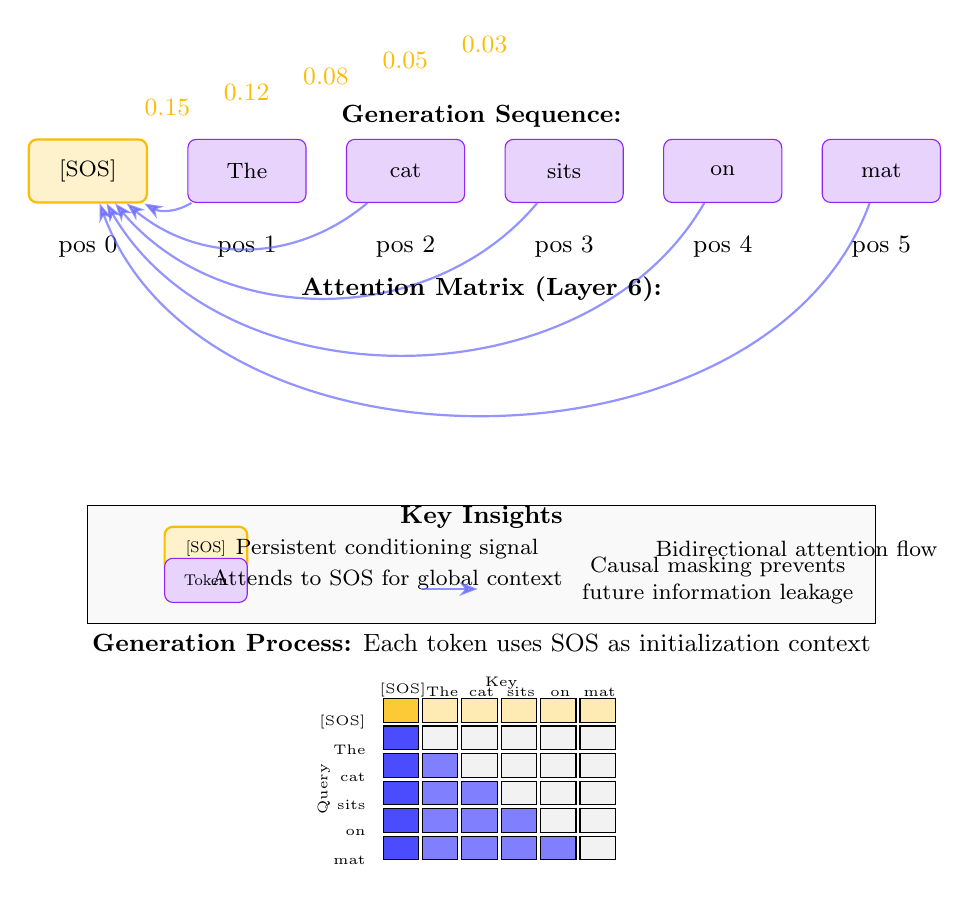
\begin{tikzpicture}[
    token/.style={rectangle, rounded corners=3pt, minimum width=1.5cm, minimum height=0.8cm, font=\footnotesize},
    sostoken/.style={token, fill=soscolor!20, draw=soscolor, thick},
    normaltoken/.style={token, fill=tokencolor!20, draw=tokencolor},
    attention/.style={-{Stealth}, thick, blue!60, opacity=0.7},
    label/.style={font=\small},
    title/.style={font=\large\bfseries}
]

% === COMPREHENSIVE SPACING AND ALIGNMENT DOCUMENTATION ===
%
% OVERALL LAYOUT (12cm width x 8cm height approximately):
% - Title: y=7.2, horizontally centered at x=6
% - Token sequence: y=6.5, spans x=1 to x=7 with 0.5cm gaps using relative positioning
% - Position labels: 0.3cm below each token using "below=0.3cm of token"
% - Attention arrows: curved paths from tokens to SOS with varying bend angles (30°-70°)
% - Attention weights: positioned along arrow curves using calc library interpolation
% - Attention matrix: y=4.5, centered at x=6 with 0.5x0.35 cell dimensions
% - Matrix labels: tiny font, positioned 0.05cm from matrix edges
% - Key insights box: y=1.5, 10cm width x 1.5cm height, centered at x=6
% - Generation process note: y=0.5, centered
%
% COLOR SCHEME:
% - SOS token: soscolor (yellow) background with soscolor border
% - Normal tokens: tokencolor (purple) background with tokencolor border  
% - SOS matrix cells: soscolor!80 (self) and soscolor!30 (column)
% - Attention matrix: blue!70 (SOS column), blue!50 (other valid), gray!10 (masked)
% - Attention arrows: blue!60 with 0.7 opacity
%
% RELATIVE POSITIONING USAGE:
% - Tokens positioned relative to previous: "right=0.5cm of previous_token"
% - Position labels: "below=0.3cm of token"
% - Matrix positioned using scope shift for grouped elements
%
% SIZE CONSTRAINTS:
% - Token minimum width: 1.5cm, height: 0.8cm with 3pt rounded corners
% - Matrix cells: 0.45x0.3cm with thin borders, 0.05cm spacing
% - Font sizes: \footnotesize for tokens, \tiny for matrix, \small for labels

% Input sequence with SOS
\node[label] at (6, 7.2) {\textbf{Generation Sequence:}};

% Tokens - using relative positioning for consistent spacing
\node[sostoken] (sos) at (1, 6.5) {[SOS]};
\node[normaltoken, right=0.5cm of sos] (t1) {The};
\node[normaltoken, right=0.5cm of t1] (t2) {cat};
\node[normaltoken, right=0.5cm of t2] (t3) {sits};
\node[normaltoken, right=0.5cm of t3] (t4) {on};
\node[normaltoken, right=0.5cm of t4] (t5) {mat};

% Position labels
\node[label, below=0.3cm of sos] {pos 0};
\node[label, below=0.3cm of t1] {pos 1};
\node[label, below=0.3cm of t2] {pos 2};
\node[label, below=0.3cm of t3] {pos 3};
\node[label, below=0.3cm of t4] {pos 4};
\node[label, below=0.3cm of t5] {pos 5};

% Attention arrows from subsequent tokens to SOS
\draw[attention] (t1) to[bend left=30] (sos);
\draw[attention] (t2) to[bend left=40] (sos);
\draw[attention] (t3) to[bend left=50] (sos);
\draw[attention] (t4) to[bend left=60] (sos);
\draw[attention] (t5) to[bend left=70] (sos);

% Attention weights (example values) - positioned along the curves
\node[label, soscolor] at ($(t1)!0.5!(sos) + (0,0.8)$) {0.15};
\node[label, soscolor] at ($(t2)!0.5!(sos) + (0,1.0)$) {0.12};
\node[label, soscolor] at ($(t3)!0.5!(sos) + (0,1.2)$) {0.08};
\node[label, soscolor] at ($(t4)!0.5!(sos) + (0,1.4)$) {0.05};
\node[label, soscolor] at ($(t5)!0.5!(sos) + (0,1.6)$) {0.03};

% Self-attention pattern visualization
\node[label] (matrix-title) at (6, 5) {\textbf{Attention Matrix (Layer 6):}};

% Create attention matrix - better positioned and sized
\begin{scope}[shift={(6,-0.5)}]
\foreach \i in {0,...,5} {
    \foreach \j in {0,...,5} {
        \ifnum\i=0
            \ifnum\j=0
                \fill[soscolor!80] (\j*0.5-1.25, -\i*0.35) rectangle ++(0.45, 0.3);
            \else
                \fill[soscolor!30] (\j*0.5-1.25, -\i*0.35) rectangle ++(0.45, 0.3);
            \fi
        \else
            \ifnum\j<\i
                \ifnum\j=0
                    \fill[blue!70] (\j*0.5-1.25, -\i*0.35) rectangle ++(0.45, 0.3);
                \else
                    \fill[blue!50] (\j*0.5-1.25, -\i*0.35) rectangle ++(0.45, 0.3);
                \fi
            \else
                \fill[gray!10] (\j*0.5-1.25, -\i*0.35) rectangle ++(0.45, 0.3);
            \fi
        \fi
        \draw[thin] (\j*0.5-1.25, -\i*0.35) rectangle ++(0.45, 0.3);
    }
}

% Matrix labels - better positioned
% Row labels (Query)
\node[label, font=\tiny, anchor=east] at (-1.35, 0) {[SOS]};
\node[label, font=\tiny, anchor=east] at (-1.35, -0.35) {The};
\node[label, font=\tiny, anchor=east] at (-1.35, -0.7) {cat};
\node[label, font=\tiny, anchor=east] at (-1.35, -1.05) {sits};
\node[label, font=\tiny, anchor=east] at (-1.35, -1.4) {on};
\node[label, font=\tiny, anchor=east] at (-1.35, -1.75) {mat};

% Column labels (Key)
\node[label, font=\tiny, anchor=south] at (-1, 0.2) {[SOS]};
\node[label, font=\tiny, anchor=south] at (-0.5, 0.2) {The};
\node[label, font=\tiny, anchor=south] at (0, 0.2) {cat};
\node[label, font=\tiny, anchor=south] at (0.5, 0.2) {sits};
\node[label, font=\tiny, anchor=south] at (1, 0.2) {on};
\node[label, font=\tiny, anchor=south] at (1.5, 0.2) {mat};

% Axis labels
\node[label, font=\tiny, rotate=90] at (-2, -0.85) {Query};
\node[label, font=\tiny] at (0.25, 0.5) {Key};
\end{scope}

% Legend
\node[rectangle, draw=black, fill=gray!5, minimum width=10cm, minimum height=1.5cm] at (6, 1.5) {};
\node[label, font=\small\bfseries] at (6, 2.1) {Key Insights};

\node[sostoken, scale=0.7] at (2.5, 1.7) {[SOS]};
\node[label, font=\footnotesize] at (4.8, 1.7) {Persistent conditioning signal};

\node[normaltoken, scale=0.7] at (2.5, 1.3) {Token};
\node[label, font=\footnotesize] at (4.8, 1.3) {Attends to SOS for global context};

\draw[attention, scale=0.7] (7.5, 1.7) -- (8.5, 1.7);
\node[label, font=\footnotesize] at (10, 1.7) {Bidirectional attention flow};

\node[label, font=\footnotesize, align=center] at (9, 1.3) {Causal masking prevents\\future information leakage};

% Generation flow
\node[label] at (6, 0.5) {\textbf{Generation Process:} Each token uses SOS as initialization context};

\end{tikzpicture}
\end{document}